% simetri-putar.tex — Ornamen simetri putar (Pak Gunanto)
% Kompilasi: pdflatex simetri-putar.tex (butuh paket tikz)
\documentclass{article}
\usepackage{tikz}
\usepackage{xcolor}
\definecolor{bgdark}{HTML}{171D2B}
\definecolor{aksen}{HTML}{F7B538}
\definecolor{aksen2}{HTML}{5B8DEF}
\pagecolor{bgdark}
\color{white}
\pagestyle{empty}
\usetikzlibrary{calc}

% Ornamen kecil: asimetris terhadap lipatan, tapi simetris terhadap putaran 180
\newcommand{\ornamen}{%
  \fill[aksen] (0,0.5) circle (0.32);
  \fill[aksen2] (0,0.5) circle (0.14);
  \fill[white] (0.55,0) circle (0.18);
  \draw[aksen,very thick] (0,0.15) -- (0,0.85);
  \draw[white,very thick] (0.15,0) -- (0.85,0);}

\begin{document}

% ---- Gambar 1: ornamen diputar 0/90/180/270 di sekitar pusat (0,0) ----
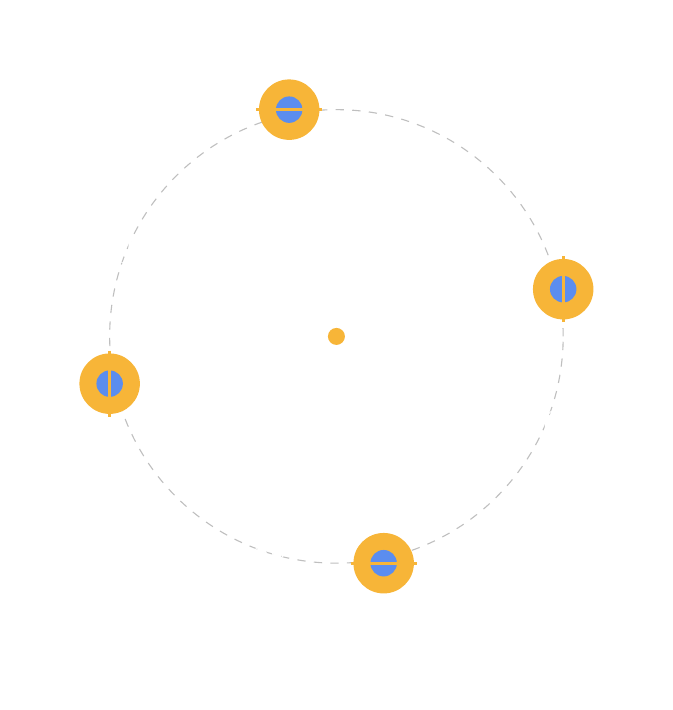
\begin{tikzpicture}[scale=1.2]
  \draw[gray!50,dashed] (0,0) circle (2.4);
  \fill[aksen] (0,0) circle (0.09);
  \foreach \a/\lbl in {0/0, 90/90, 180/180, 270/270}{
    \begin{scope}[rotate=\a]
      \begin{scope}[shift={(2.4,0)}] \ornamen \end{scope}
      \node[white,font=\LARGE] at (2.4,-0.95) {\lbl$^\circ$};
    \end{scope}}
  \node[white,font=\large] at (0,-3.4) {pusat putar di titik yang sama};
\end{tikzpicture}

\clearpage

% ---- Gambar 2: kawung, simetri putar orde 4 ----
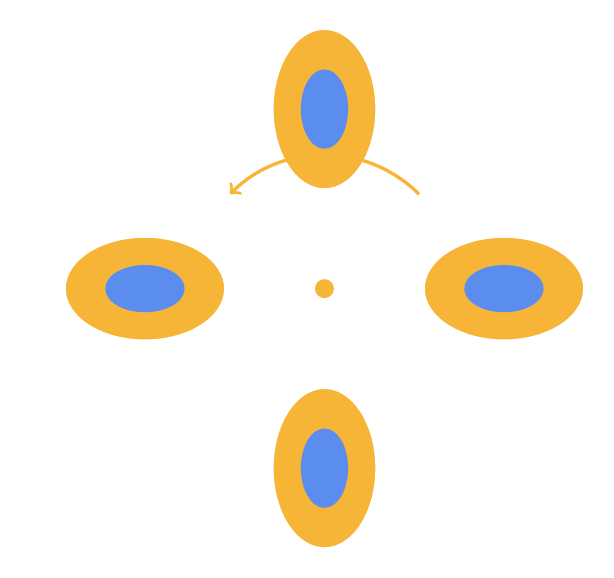
\begin{tikzpicture}[scale=1.2]
  \fill[aksen] (0,0) circle (0.10);
  \foreach \a in {0,90,180,270}{
    \begin{scope}[rotate=\a]
      \fill[aksen] (0,1.9) ellipse (0.55 and 0.85);
      \fill[aksen2] (0,1.9) ellipse (0.25 and 0.42);
      \draw[white,thick] (0,1.9) ellipse (0.55 and 0.85);
    \end{scope}}
  % panah arah putaran
  \draw[aksen,very thick,->] (1.0,1.0) arc (45:135:1.414);
  % label sudut di dekat tiap posisi petal
  \node[white,font=\LARGE] at (2.0,2.4)  {$0^\circ$};
  \node[white,font=\LARGE] at (-2.4,2.4) {$90^\circ$};
  \node[white,font=\LARGE] at (-2.6,-2.0){$180^\circ$};
  \node[white,font=\LARGE] at (2.0,-2.0) {$270^\circ$};
\end{tikzpicture}

\end{document}
